\chapter{The LAGUNA-LBNO Experiment}
LAGUNA-LBNO (Large Apparatus studying Grand Unification and Neutrino Astrophysics and Long Baseline Neutrino Oscillations) is a feasibility study for the design and implementation of  a next generation neutrino experiment \cite{laguna1}. With the existence of massive neutrinos showing the only experimentally observed deviation from the Standard Model, they can be key to probing our deeper understanding of the universe. The experimental project of LAGUNA-LBNO is discussed in this chapter to give an overview of the aims, setup and its relevance to neutrinos. 

\section{The CERN-Pyh\"{a}salmi Baseline}
The LAGUNA-LBNO experiment consists of a neutrino beam originating from a facility within CERN (European Organisation for Nuclear Research) in Geneva, aimed to a Far Detector based in Pyh\"{a}salmi, Finland, at a distance of 2300 km away. A Near Detector (ND) of gas argon technology is proposed while the FD technology is uncertain with either liquid argon, Water Cherenkov or liquid scintillator design suggested, respectiviely GLACIER \cite{GLACIER}, MEMPHYS \cite{MEMPHYS} and LENA \cite{LENA}.

The Pyh\"{a}salmi mine in Finland is the host site for the FD and at -1440 m the mine is the deepest in Europe, allowing unique opportunities for neutrino and astrophysics. With an extremely large baseline of 2300 km neutrino oscillation matter effects are no longer negligible and can be exploited to determine the mass hierarchy of neutrinos. It can also provide the most accurate measurement of the CP-violating phase factor, $\delta$, given that $\theta_{13}$ is now found to be large. With a distance close to the bimagic baseline\cite{magicBaseline1} it puts us in a unique position to exploit the $P(\nu_{\mu} \to \nu_{e})$ transition. Figure \ref{fig:baselineProbFig} shows the appearance channel as a function of incoming neutrino energy for the CERN-Pyh\"asalmi baseline, with oscillation parameters from table \ref{tab:osciParameterTable} used. The two hierarchies are shown with varying values for $\delta$. The vacuum oscillation is also plotted for which matter effects are not considered and shows the 1$^{st}$ oscillation maximum around 4.6 GeV. The difference between the two hierarchies becomes apparent above 4 GeV when using matter effects, regardless of the value of $\delta$. Figure \ref{fig:baselineProb2Fig} shows the $P(\nu_{\mu} \to \nu_{\mu})$ transition and it can be seen that it is independent of $\delta$, so to measure CP-violation the appearance channel must be used. 

\begin{figure}[htbp]
\begin{center}
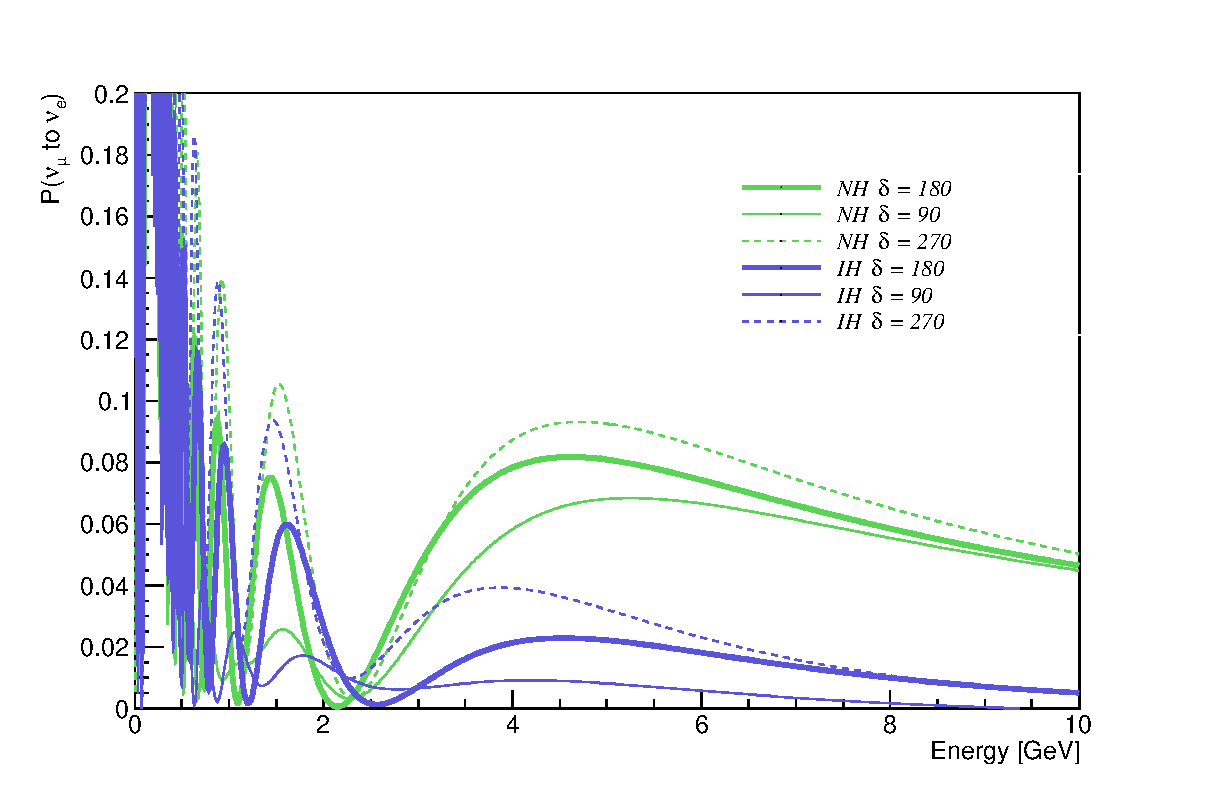
\includegraphics[width=90mm]{Chapter2/figures/numu_nue_matter_effects.eps}
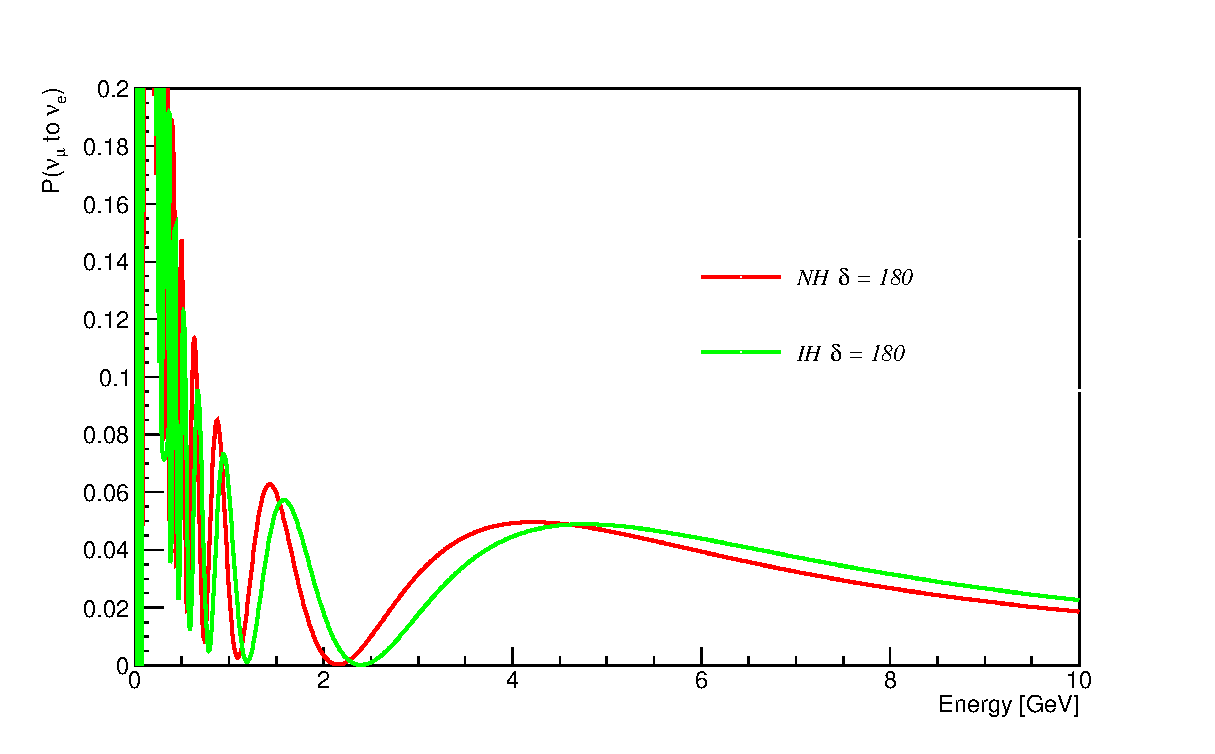
\includegraphics[width=90mm]{Chapter2/figures/numu_nue_no_matter_effects.eps}
\caption{The appearance channel probability as a function of incoming neutrino energy for the Pyh\"asalmi baseline with matter effects (upper) and without (lower).}
\label{fig:baselineProbFig}
\end{center}
\end{figure}

\begin{figure}[htbp]
\begin{center}
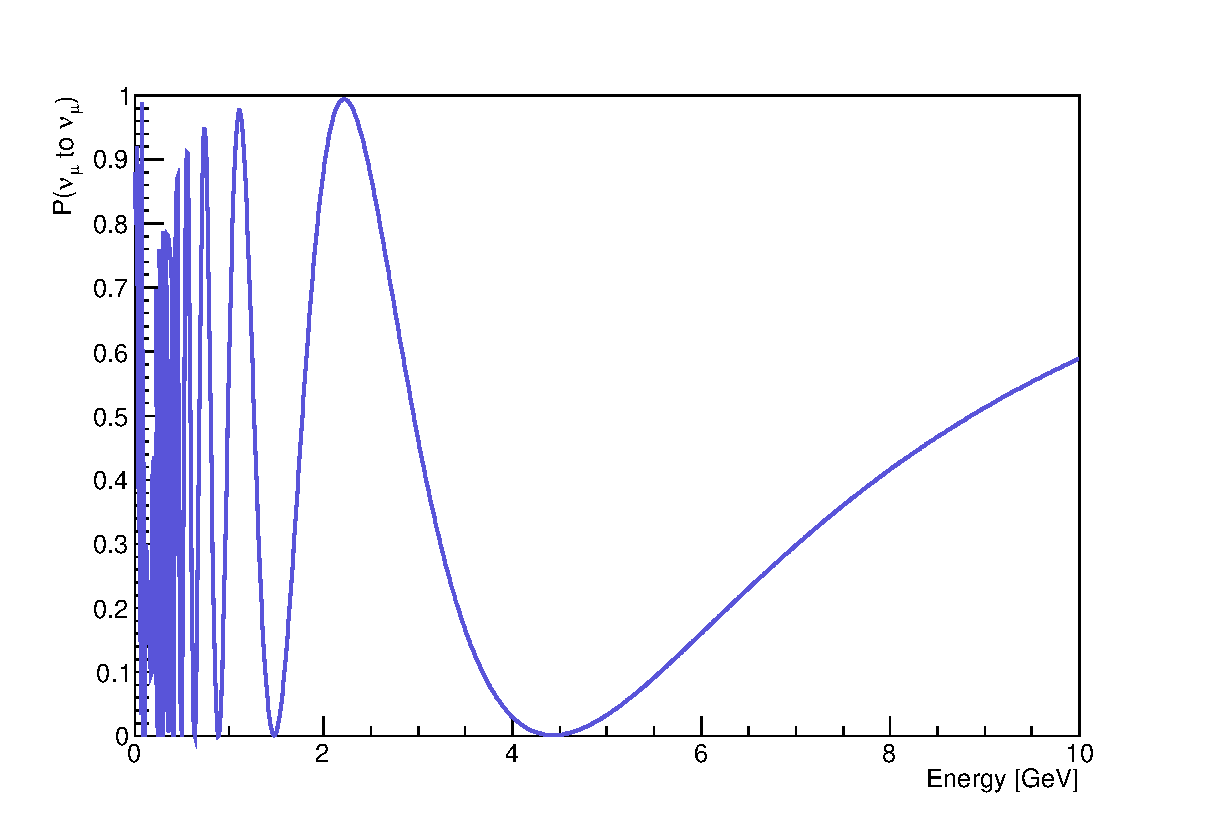
\includegraphics[width=90mm]{Chapter2/figures/numu_numu.eps}
\caption{The disappearance channel probability as a function of incoming neutrino energy for the Pyh\"asalmi baseline for which is independant of $\delta_{CP}$.}
\label{fig:baselineProb2Fig}
\end{center}
\end{figure}

To quantify CP violation is it useful to define asymmetries between the oscillation probabilities for neutrinos and antineutrinos. These are given for vacuum and matter probabilities in equations \ref{eq:cpAsymmVacumm} and \ref{eq:cpAsymmMatter} respectively. These two asymmetry variables are plotted in the neutrino energy against baseline plane and are shown in figure \ref{fig:cpvSensitivity} \cite{lbnoEoI} for fixed values of $\delta_{CP}$ = 270 \textdegree and Earth matter density of 2.8 gcm$^{-3}$. At 2300 km clear separation between the first and second maxima is noticeable and achievable for a wide band beam.

\begin{equation}
	A_{CP}^{vac}(\delta_{CP}) = abs \left(\frac{P^{vac}(\nu) - P^{vac}(\bar{\nu})}{P^{vac}(\nu) + P^{vac}(\bar{\nu})}\right)
	\label{eq:cpAsymmVacumm}
\end{equation}
\begin{equation}
	A_{CP}^{mat}(\rho) = abs \left(\frac{P^{mat}(\nu) - P^{mat}(\bar{\nu})}{P^{mat}(\nu) + P^{mat}(\bar{\nu})}\right)
	\label{eq:cpAsymmMatter}
\end{equation}

\begin{figure}[htbp]
\begin{center}
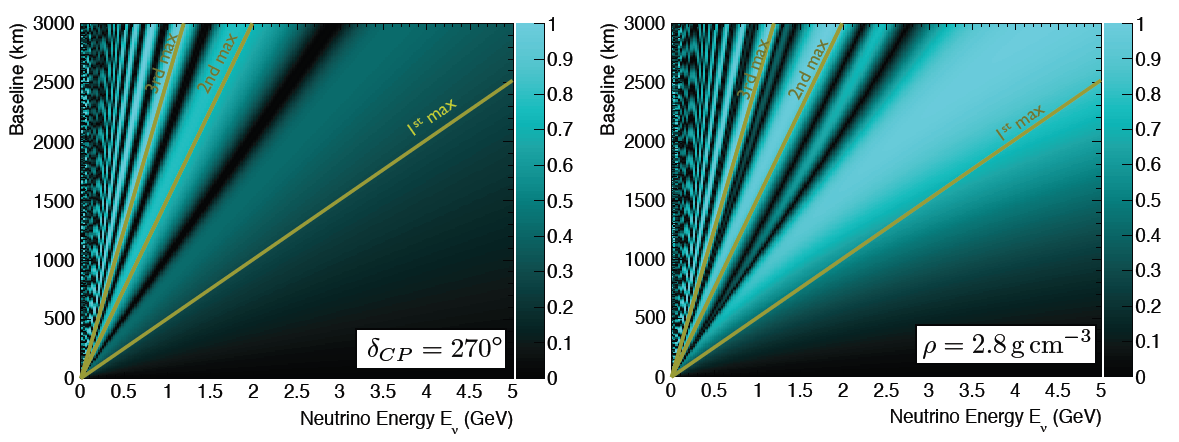
\includegraphics[width=160mm]{Chapter2/figures/cpvSensitivity.png}
\caption{The two asymmetries in vacuum (left) and in matter (right) of density 2.8 gcm$^{-3}$ as a function of neutrino energy and baseline. First, second and third maxima are shown for constant L/E values. Plots taken from \cite{lbnoEoI}. }
\label{fig:cpvSensitivity}
\end{center}
\end{figure}

Considering that the Pyh\"asalmi site provides the largest baseline of the seven, the required neutrino energy must be large due to the $L/E$ optimisation. This baseline does not favour MEMPHYS, as Water Cerenkov detectors are used for energies below the 1 GeV region.  In this energy region CCQE events dominate and Water Cerenkov's can reconstruct such events well, with general CCQE events producing a single ring for muons and multiple rings for electrons. For the energies required for a 2300 km baseline with 1$^{st}$ oscillation maximum at 4.6 GeV, dominant processes are then resonance (RES) and Deep Inelastic Scattering (DIS). This is not favourable to Water Cerenkov technology as this produces large amounts of rings which cannot be reconstructed. Liquid Scintillator poses to overcome these problems with current studies \cite{LENA} arguing that reconstruction can work for energies above 1 GeV, although this technology is limited by Neutral Current (NC) backgrounds. The technology that is preferred for such a baseline is the LAr detector, GLACIER, due to its reconstruction properties at high energies.

\section{Physics Potential}
The 2300 km baseline coupled with the GLACIER detector offers a rich and broad physics program for neutrino oscillations and other particle physics studies, including nucleon decay searches. In terms of neutrino physics the LAGUNA-LBNO experiment offers unrivalled opportunities to precisely measure and resolve the neutrino mass hierarchy, reaching this to beyond a 5$\sigma$ confidence level (C.L) within $\sim$4 years of running \cite{lbnoInternal}, shown in figure \ref{fig:massHierarchyPlots}. It also has the potential to discover evidence for CP violation in the leptonic sector, with a 20 ktonne GLACIER detector covering $\sim$45\% of possible CP values at 3$\sigma$ C.L. This is shown in figure \ref{fig:cpvReachPlots}. Current experiments like T2K and NO$\nu$A are less sensitive to these effects due to shorter baselines and lower neutrino energies.

\begin{figure}[htbp]
\begin{center}
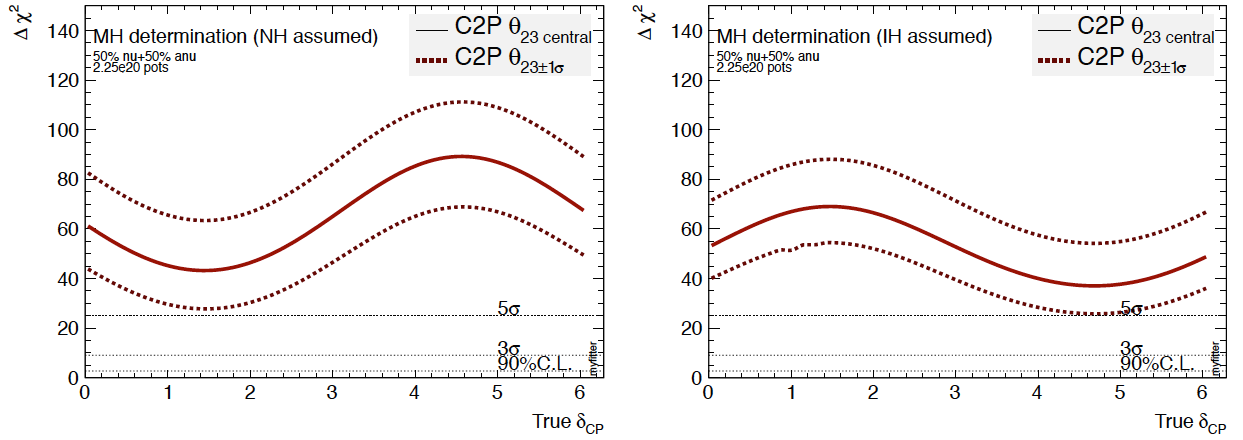
\includegraphics[width=150mm]{Chapter2/figures/massHierarchyPlots.png}
\caption{The mass hierarchy determination for normal (left) and inverted (right) hierarchies. Showing in excess of a 5$\sigma$ C.L for both cases. Plots taken from \cite{lbnoInternal}.}
\label{fig:massHierarchyPlots}
\end{center}
\end{figure}
\vspace{-5mm}
\begin{figure}[htbp]
\begin{center}
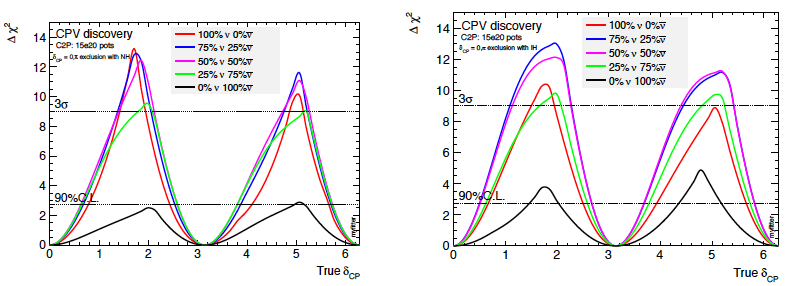
\includegraphics[width=150mm]{Chapter2/figures/cpvReach.png}
\caption{The CPV sensitivity for various $\nu$ and $\bar{\nu}$ beam sharing modes for a 20 ktonne GLACIER detector. The different contours show the CPV discovery potential for various levels of beam sharing modes ($\nu$,$\overline{\nu}$), red indicates (100\%,0\%), blue (75\%,25\%), purple (50\%,50\%), green (25\%,75\%), black(0\%,100\%). The left plot shows the discovery potential for NH with the right plot showing it for the IH. Plots taken from \cite{lbnoInternal}.}
\label{fig:cpvReachPlots}
\end{center}
\end{figure}

\section{Generating Neutrinos}
Unlike solar, atmospheric and reactor neutrino oscillation measurements, long baseline oscillation experiments are tailored to the physics requirements, where neutrinos are created and controlled at a source. Neutrinos are generated from the decay of short lived particles, and depending on the type of the parent particle then defines the neutrino beam type. Conventionally, high energy protons are fired into a target to create secondaries, consisting of charged mesons, which in turn decay into neutrinos. This is a conventional neutrino beam. The dominant decay chain from this type of beam is,
\begin{equation}
\pi^{\pm} \rightarrow \mu^{\pm} + \overset{(-)}{\nu}_{\mu}
\end{equation}
but it is also possible to have,
\vspace{-4mm}
\begin{equation}
\pi^{\pm} \rightarrow e^{\pm} + \overset{(-)}{\nu}_{e}
\end{equation} 
however this decay mode is helicity suppressed and has a small branching ratio measured as (1.230 $\pm$ 0.004) $\times$ 10$^{-4}$ \cite{pionDecayModes}. Kaons can also decay via these chains generating a leptonic pair of a muon and neutrino, however they can also decay via other modes involving three body decays, generating larger amounts of electron neutrinos. Table \ref{tab:kaonDecayModes} shows the main decay modes with their corresponding branching ratios observed from experiments \cite{kaonDecayModes}. 
\begin{table}[htbp]
\begin{center}
  \begin{tabular}{l*{2}{c}r}
  \hline
  \textbf{Decay Mode} & \textbf{Branching Ratio (\%)}\\
    \hline
    \hline
    $\mu^{+}\boldsymbol{\nu_{\mu}}$ & 63.55 $\pm$ 0.11\\
    $\pi^{+}\pi^{0}$ & 20.66 $\pm$ 0.08\\
    $\pi^{+}\pi^{+}\pi^{-}$ & 5.59 $\pm$ 0.04\\
    $\pi^{0}e^{+}\boldsymbol{\nu_{e}}$ & 5.07 $\pm$ 0.04\\
    $\pi^{0}\mu^{+}\boldsymbol{\nu_{\mu}}$ & 3.353 $\pm$ 0.034\\
    $\pi^{+}\pi^{0}\pi^{0}$ & 1.761 $\pm$ 0.022\\
    \hline
  \end{tabular}
      \caption{The main decay modes (>1\%) of K$^{+}$ with its corresponding branching ratios. K$^{-}$ decay modes are the same but are charge conjugated. Data taken from \cite{kaonDecayModes}.}
    \label{tab:kaonDecayModes}
\end{center}
    \end{table}
    
Muons produced from these mesons can decay before being stopped and they introduce further contamination to the beam via
\begingroup
  \addtolength\abovedisplayskip{-0.5\baselineskip}%
  \addtolength\belowdisplayskip{-0.7\baselineskip}%
 \addtolength\abovedisplayshortskip{-0.5\baselineskip}%
 \addtolength\belowdisplayshortskip{-0.1\baselineskip}%
\begin{equation}
\mu^{-}  \rightarrow e^{-} + \overline{\nu}_{e} + \nu_{\mu} 
\end{equation}
\vspace{-2mm}
\begin{equation}
\mu^{+}  \rightarrow e^{+} + \nu_{e} + \overline{\nu}_{\mu}.
\end{equation}
\endgroup
Contaminations of other neutrino flavours can cause problems for oscillation searches due to these wrong flavour neutrinos reaching the far detector.

Neutrino factories aim to remove this contamination by using only the decays of muons to create neutrinos. From the pion decays, muons are collected in storage rings and accelerated to the desired momentum. They are then optimised for $\nu_{\mu} \rightarrow \nu_{e}$ and $\overline{\nu}_{\mu} \rightarrow \overline{\nu}_{e}$ searches as a magnetised detector can then identify the sign of the muon and hence measure oscillation parameters. Unfortunately currently neutrino factories are a relatively new idea and are extremely expensive. Ongoing studies are working towards developing the technology and maximising their sensitivities but there is no immediate demand to implement these beams in the near future. This technology would indeed provide a very clean beam and dramatically reduce the systematical uncertainties that arise from the beam, but as $\theta_{13}$ has recently been measured to be non-zero makes the mass hierarchy and CP violation accessible with conventional beams.

%Other than the steep costs of such a technology requires, there is no urgent demand within the current climate as $\theta_{13}$ has now been measured to be non zero to greater than 5$\sigma$. Although neutrino factories provide a very clean beam and dramatically reduce the systematical uncertainties from the beam,  but with the $\theta_{13}$ now measured to be non zero to greater than 5$\sigma$ such .

\section{The Beam Facility}
LAGUNA-LBNO proposes to use a conventional neutrino beam approach from a new facility Cern Neutrinos to Pyh\"asalmi (CN2PY). The current layout of the main accelerators at CERN are shown in figure \ref{fig:cernLayout}. Two beam options exist, a 50 GeV proton extraction from a newly proposed synchrotron, the High Power Proton Synchrotron (HP-PS) or 400 GeV proton extraction from the existing Super Proton Synchrotron (SPS) beam line at CERN. Both Positive Focusing (PF) and Negative Focusing (NF) options are required for each beam line yielding $\nu_{\mu}$ and $\bar{\nu}_{\mu}$ runs respectively.

\begin{figure}[ht]
\begin{center}
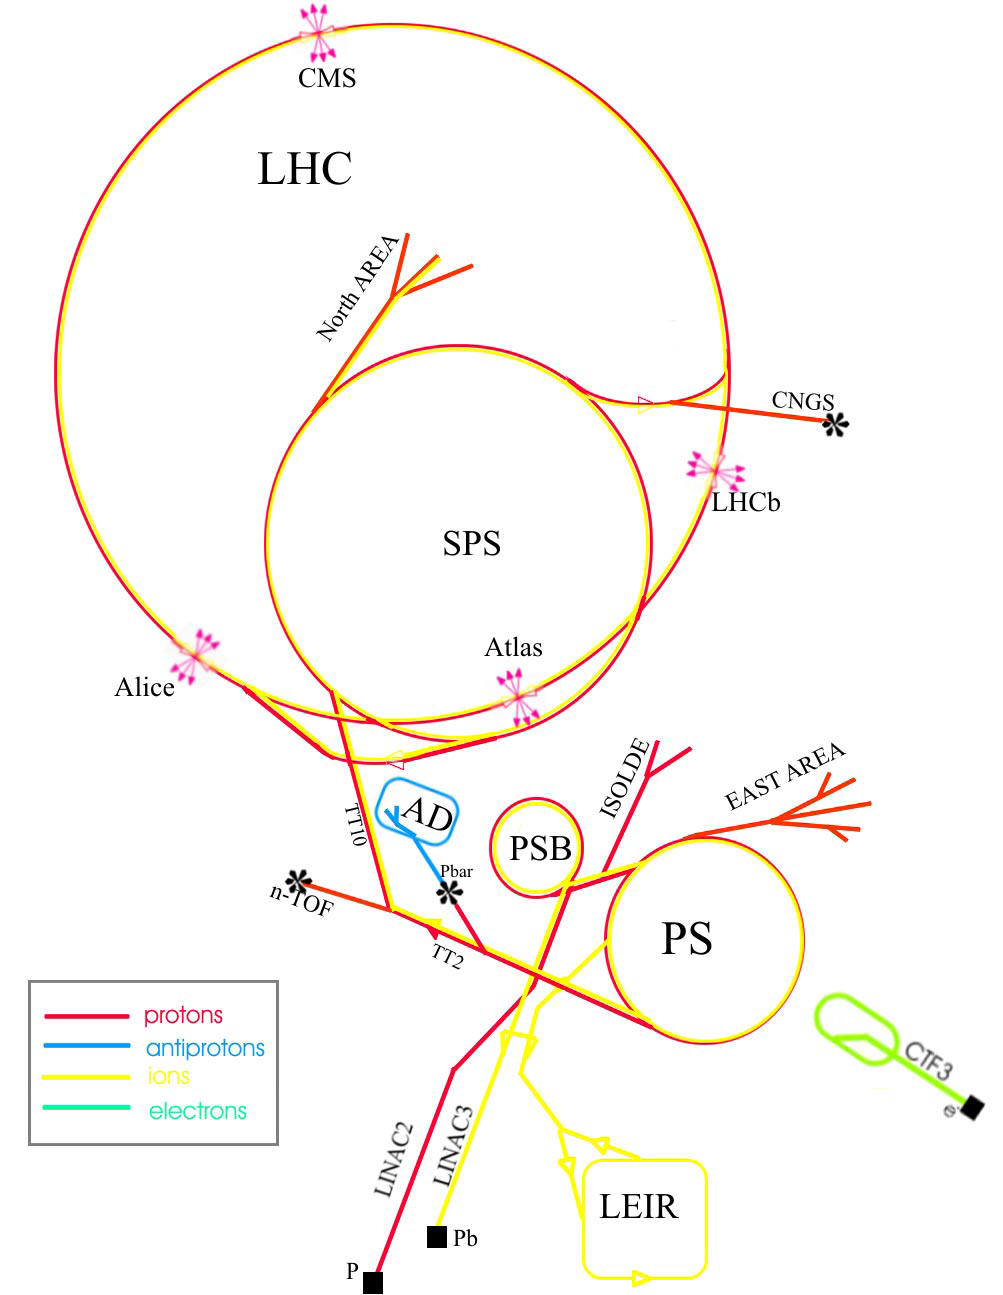
\includegraphics[width=90mm,height=110mm]{Chapter2/figures/cernBeamLayout.jpg}
\caption{The accelerator and beam complex at CERN. Image from \cite{cernBeamLayoutPic}.}
\label{fig:cernLayout}
\end{center}
\end{figure}

\subsection{400 GeV Option}
The first step in the beam is the Linear Accelerator 2 (Linac 2), consisting of cylindrical conductors operating at radio frequency. Protons are created from a hydrogen gas source at one end of the Linac 2, by initially passing the hydrogen through an electric field the removal of its electrons leaves only the protons. The protons are then accelerated to energies of 50 MeV upon reaching the other end of the Linac 2. Small quadrupole magnets are required to ensure that the beam is kept tight. The protons are extracted in pulses from the hydrogen source over periods of up to 100$\mu$s per pulse. 

Upon leaving the Linac 2, they then enter the Proton Synchrotron Booster (PSB) to increase their energy. The PSB consists of four superimposed synchrotron rings which accelerate the protons to 1.4 GeV for injection into the Proton Synchrotron (PS). The PS then accelerates the protons to 25 GeV to which they are subsequently injected into the SPS to reach energies of 400 GeV, at which point they are extracted from the SPS.

It is proposed that per 10.5 $\mu$s extraction from the SPS a rate of 7 $\times$ 10$^{13}$ protons on target (p.o.t) per proton pulse (ppp) can be achieved. This is based on two extractions per 6 s cycle of 3.5 $\times$ 10$^{13}$ p.o.t from the SPS, separated by 50 ms intervals. The corresponding instantaneous SPS beam intensity is then $\sim$1.2 $\times$ 10$^{13}$ protons per second at 400 GeV, equivalent to a beam power of $\sim$750 kW.

Assuming a pessimistic operation with 60\% beam sharing, 85\% accelerator efficiency and yearly run period of 200 days its expected to obtain $\sim$1.0 $\times$ 10$^{20}$ p.o.t / year \cite{lbnoEoI}.

\subsection{50 GeV Option}
The 50 GeV option relies on the new Linear Accelerator (Linac 4) which is expected to be completed for 2018. This will use negative Hydrogen ions (H$^{-}$), which are Hydrogen atoms with an additional electron, as the source. Again the electrons will be removed upon passing an electric field but this will accelerate them to 160 MeV. Besides the higher proton energy, the Linac 4 will allow more protons to accumulate with a simpler injection and therefore provide a better beam.

Upon leaving the Linac 4, the protons are injected into the High-Power Proton Synchrotron (HP-PS) upon which they are accelerated to 50 GeV. This design is very much in progress with technical studies ongoing, however some basic estimations can be made. It is assumed that a beam power of 2 MW can be achieved with 2.5 $\times$ 10$^{14}$ ppp and a superior extraction rate of 1 Hz compared to the 400 GeV option.

\subsection{Layout}
Both beam options require similar design layouts, although there is a higher level of uncertainty for the 50 GeV option due to the location of the HP-PS. The beam layout for the 400 GeV option is discussed only, as this is beam option of choice for the majority of the studies in this thesis. The proposed location for the beam facility is in the north area of CERN, and it can be seen in figure \ref{fig:beamLocation} where the extraction point and ND will be placed.

\begin{figure}[htbp]
\begin{center}
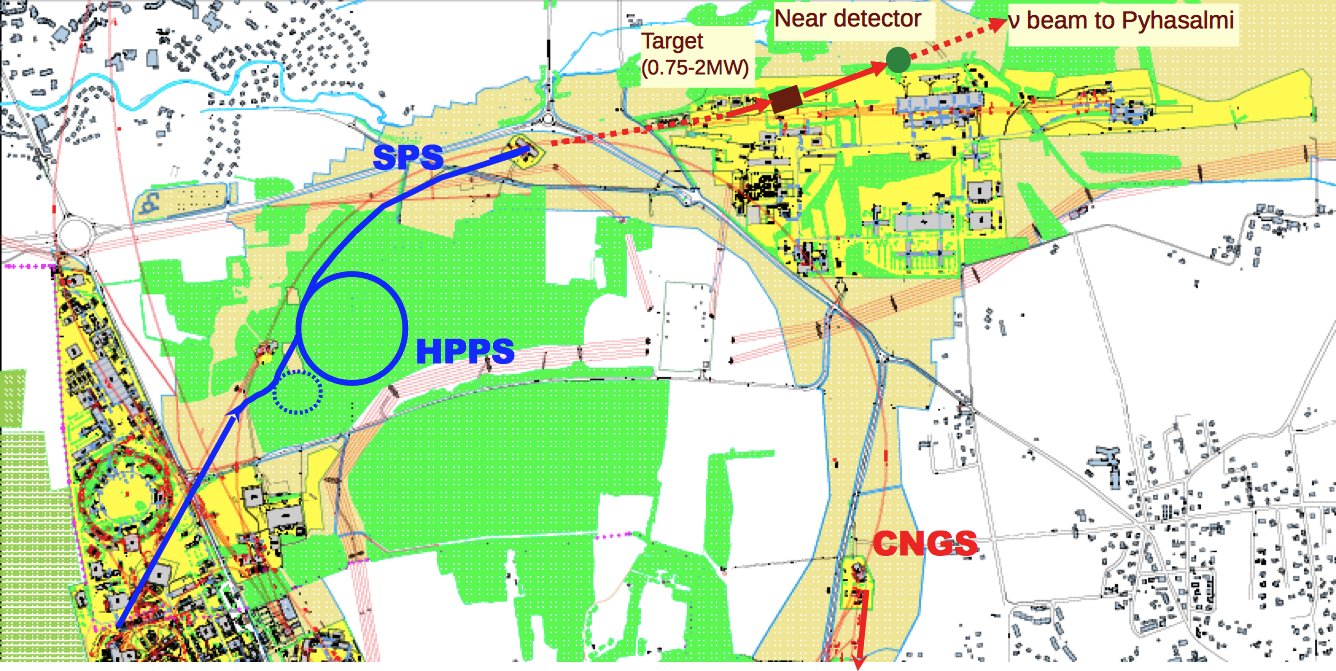
\includegraphics[width=140mm]{Chapter2/figures/beamPlacement.png}
\caption{The expected location for the beam facilities and ND in the north area of CERN \cite{lbnoInternal}.}
\label{fig:beamLocation}
\end{center}
\end{figure}

\subsection{Design}
A 10.4$^{\circ}$ inclination angle is required to reach the Pyh\"asalmi site, after extraction from the SPS the protons are bent to this angle shortly before hitting the beam target. A 1 m long graphite cylinder of density 1.85 gcm$^{-3}$ and radius of 2 mm forms the beam target. Shortly after the target magnetic parabolic horns are used to focus the secondaries into the decay pipe. The horns are optimised primarily for the $\nu_{\mu}$ energy at the first oscillation maximum, with consideration to incorporate the flux at the second oscillation maximum also, at 1.44 GeV. 

A 300 m long decay pipe allows for the decay of the mesons produced with a hadron stop at the end of the pipe to collect all non decayed hadrons. With muons passing through the hadron stop a muon monitor is placed at 30 m downstream to this in order to measure the muon flux.

The path the neutrinos will follow to Pyh\"asalmi can be seen in figure \ref{fig:neutrinoPathInRock}. This shows the estimated matter composition and approximate densities of the Earth's crust according to geological studies \cite{neutrinoPathInRock}.

\begin{figure}[htbp]
\begin{center}
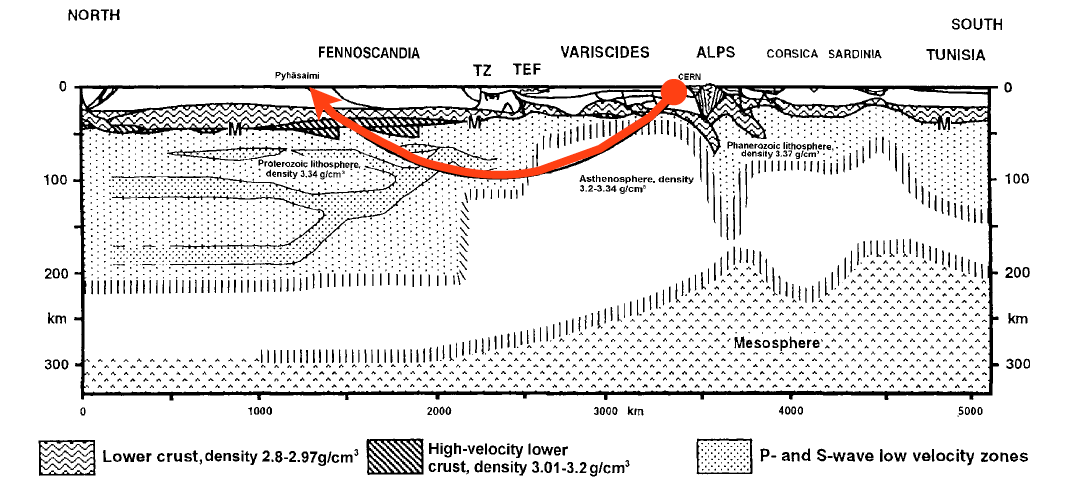
\includegraphics[width=140mm]{Chapter2/figures/neutrinoPathInRock.png}
\caption{The path of the neutrinos from CERN to Pyh\"asalmi (red) shown against the main tectonic elements of Western Europe with the corresponding densities \cite{neutrinoPathInRock}\cite{lbnoInternal}.}
\label{fig:neutrinoPathInRock}
\end{center}
\end{figure}

\section{The Expected Neutrino Flux}
Following from the implementation of the beam design into the simulation package FLUKA\cite{fluka}, the unoscillated neutrino fluxes expected at the FD can be determined as a function of neutrino energy. The expected neutrino flux at both the ND (placed at 800 m from the target, 3 m radius cut) and FD (2300 km from the target and 1 km radius cut) is then shown in figure \ref{fig:neutrinoFluxNearAndFar} for both beam options and positive focusing runs. Each beam option is normalised to the beam power. It can be noticed that for both beam options the fluxes at both the near and far detectors are very similar in shape and hence will provide a fairly constant Near/Far ratio.

\begin{figure}[hbtp]
	\begin{center}
		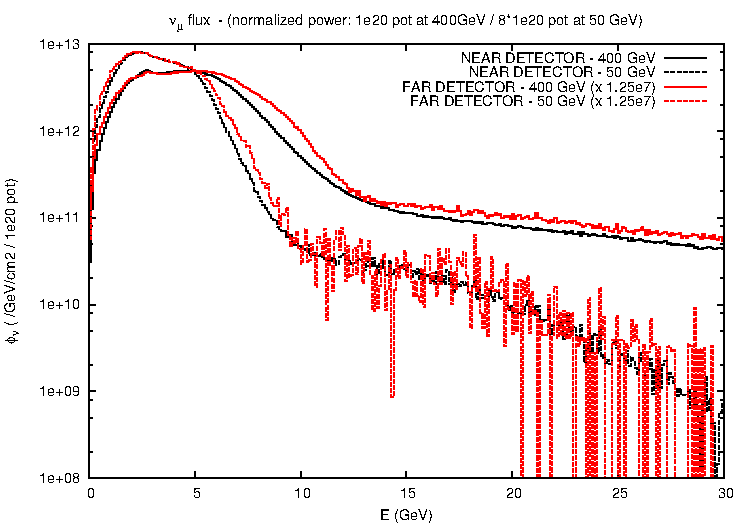
\includegraphics[width=74mm]{Chapter2/figures/numu_ND_FD.pdf}
		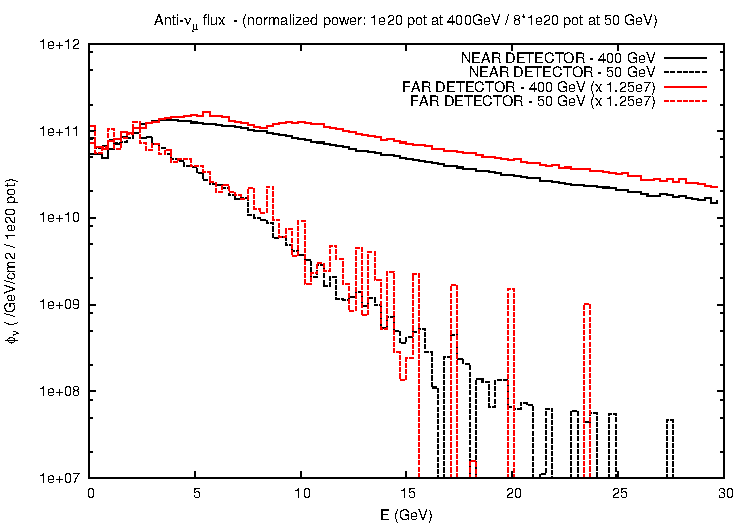
\includegraphics[width=74mm]{Chapter2/figures/anumu_ND_FD.pdf}
		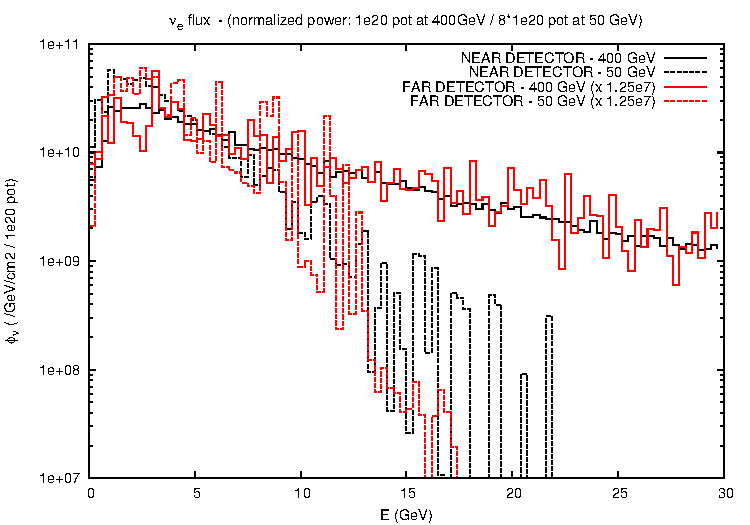
\includegraphics[width=74mm]{Chapter2/figures/nue_ND_FD.pdf}
		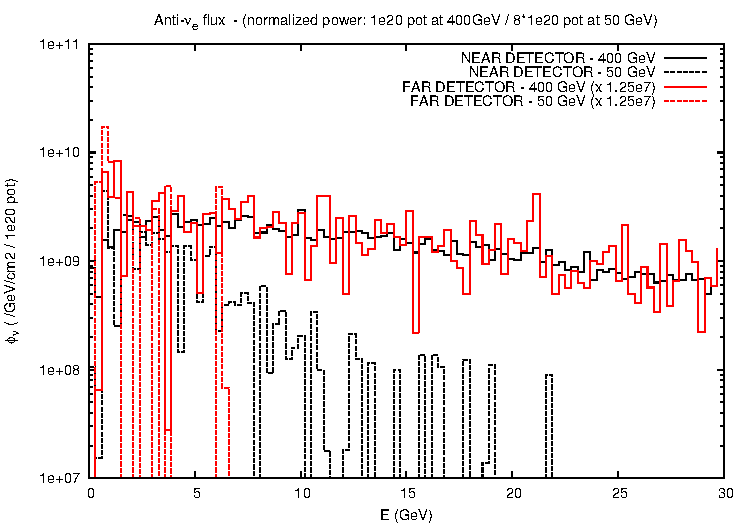
\includegraphics[width=74mm]{Chapter2/figures/anue_ND_FD.pdf}
	\caption{Clockwise from top left: $\nu_{\mu}$, $\overline{\nu}_{\mu}$, $\overline{\nu}_e$ and $\nu_e$ spectra for horns set to positive focusing ($\nu_{\mu}$ run). Both beam options, 50 and 400 GeV beams are shown for near and far detectors (unoscillated) with a 3 m and 1 km radius cut respectively. The beams are normalised to equivalent beam power \cite{lbnoInternal}\cite{lbnoNDTechNote}.}
	\label{fig:neutrinoFluxNearAndFar}
\end{center}
\end{figure}

\section{The Near Detector}
Fundamentally the ND is required to perform measurements on the neutrinos before oscillation and is used to extrapolate the flux to the FD. This however introduces systematic errors but which can be reduced by matching target materials of both near and far detectors. A Gas Argon (GAr) TPC design in proposed as the ND and the feasibility of such an instrument is the focus of this thesis. GAr is chosen as the target material instead of its liquid counterpart due to its lower density ($\sim$40 times less at 20 bar), resulting in fewer neutrino interactions in the ND and avoiding pile up, improved charged track reconstruction and also benefits from the lack of cryogenics. However implementing a pressurised GAr TPC introduces some technical and engineering problems that must be also be considered. Details of the ND are covered in the following chapter.

With the ND completing the facilities at CERN a summary of the estimated distances of each instrument is shown in table \ref{tab:cernFacility}. 

\begin{table}[htbp]
\begin{center}
  \begin{tabular}{l*{2}{c}r}
  \hline
  \textbf{Component} & \textbf{Distance [m]} & \textbf{Depth [m]} \\
    \hline
  \hline
    Beam Target & 0 & 0 \\
    Hadron Stop & 300 & -54.2 \\
    Muon Monitor & 330 & -59.6 \\
    Near Detector & 800 & -144.4 \\
    \hline
  \end{tabular}
      \caption{The relative distances and depths for each beam and detector component at the CERN facility.}
    \label{tab:cernFacility}
\end{center}
    \end{table}

\section{The Far Detectors}
\subsection{GLACIER}
An incremental approach is taken for the FD design, initially considering a 20 ktonne detector, with 50 ktonne and 100 ktonne options available for future upgrades. However due to cavern excavation restrictions, a cavity big enough to host a 100 ktonne detector is not possible, so it would comprise of two 50 ktonne detectors. The 20 ktonne detector is assumed for this study and its concept is described. Larger volumes would follow from this design with all three sizes employing a 20 m drift distance but with larger volumes having increased vessel diameters.

The 20 ktonne GLACIER detector is of cylindrical design, with the flat ends forming the top and bottom of the detector, with the design shown in figure \ref{fig:glacierDesignInner}. The inner vessel diameter of 37 m and inner height of 22 m yields a volume of 23654.6 m$^{3}$ of Argon. At a depth of 1400 m in the Pyh\"asalmi mine the pressure is approximately 1.2 bar, this corresponds to a density of 1.38 gcm$^{-3}$ for liquid Argon. The total mass is then 32.7 ktonnes assuming constant density across the whole volume. An active instrumented mass of the detector is then 22.8 ktonnes. \cite{lbnoEoI}. Due to hydrostatic pressure of the Argon in the vessel the pressure on the bottom of the vessel is 4.2 bar.

The detector operates in double-phase (liquid-vapor) using charge readout and amplification in the vapour phase. An octagonal field cage creates a uniform electric field in the vertical direction. The cage is composed of equally spaced stainless steel rings which are held in place with a series of mechanical structures. The support structure is then suspended by stainless steel ropes from the outer deck of the detector. To acquire drift velocities of electrons at $\sim$2 mm/$\mu$s a field strength of 1 kV/cm is required. Over a 20 m drift distance this corresponds to a high voltage of 2MV. 
%Such high voltages are achievable in liquid Argon based on the Grienacher HV multiplier [ref here].

The charge is read out at the top of the detector which also functions as the anode, with the cathode at the bottom of the tank. The charge readout consists of 804 square panels, each of 1 m$^{2}$ and 40 triangular panels of 0.5 m$^{2}$ for the curved ends. 416 signal feedthroughs are required to channel the readout signals, these are located in the roof of the vessel.

In addition to charge readout the design implements the collection of scintillation light also, with an array of PMTs placed below the cathode. One 8$^{\verb+"+}$ PMT is placed per 1 $\times$ 1 m$^{2}$ area, resulting in 804 PMTs on the base of the vessel. They each have a buoyancy of $\sim$4 kg in liquid Argon and are anchored to the bottom of the tank to compensate for this. They must also be able to withstand the 4.2 bar hydrostatic pressure. 

\begin{figure}[htbp]
\begin{center}
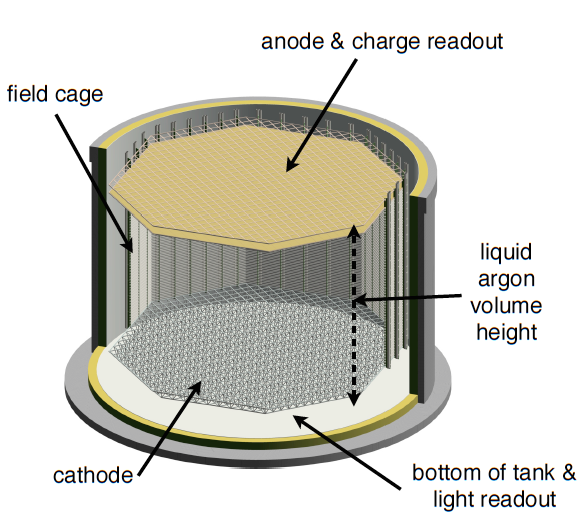
\includegraphics[width=70mm]{Chapter2/figures/glacierDesignOpen1.png}
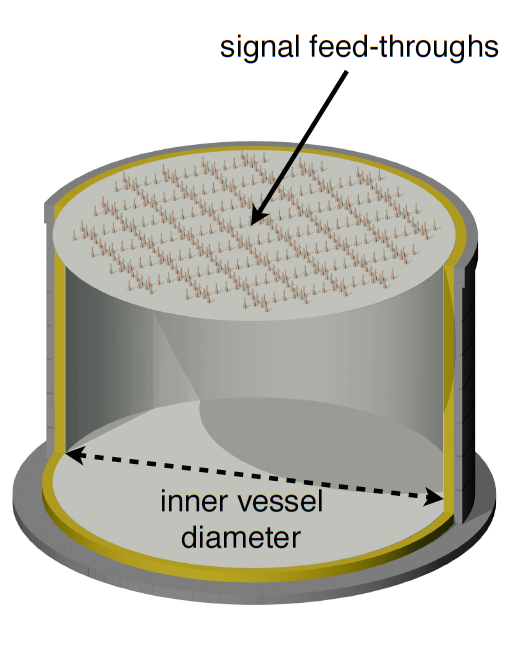
\includegraphics[width=50mm]{Chapter2/figures/glacierDesignOpen2.png}
\caption{The labelled components of the GLACIER detector design. Image from \cite{lbnoInternal}.}
\label{fig:glacierDesignInner}
\end{center}
\end{figure}

\subsection{Magnetised Iron Neutrino Detector}
The Magnetised Iron Neutrino Detector (MIND) is also proposed as a FD in addition to GLACIER. It is a sampling calorimeter consisting of alternating iron and scintillator layers. This follows from the MINOS detector design \cite{minosExperiment}, which is a well proven technology for neutrino detection. It is proposed to complement the primary FD as, unlike GLACIER, it is magnetised so it can perform charge identification and momentum measurements. The majority of high energy muons (>5 GeV) produced from neutrino interactions in the Argon will not be contained within the GLACIER detector. Placement of the MIND downstream of the GLACIER detector is then necessary.

A 40 m $\times$ 20 m $\times$ 10 m MIND is considered, with a width and height to match that of the GLACIER detector. Each iron layer is of 3 cm thickness and each scintillator layer thereafter is 2 cm thick. This corresponds to a mass of $\sim$38 ktonne of iron and $\sim$9 ktonne of scintillator if a box shape is employed. Values and parameters of the design are at a preliminary stage as little effort has been put into the MIND design. It is estimated that a magnetic field strength of between 1.5 and 2.5 T is required \cite{lbnoInternal}. A sketch of the design is shown in figure \ref{fig:mindFD} with its proposed integration with the GLACIER detector shown in figure \ref{fig:glacierMindLayout}.

\begin{figure}[htbp]
\begin{center}
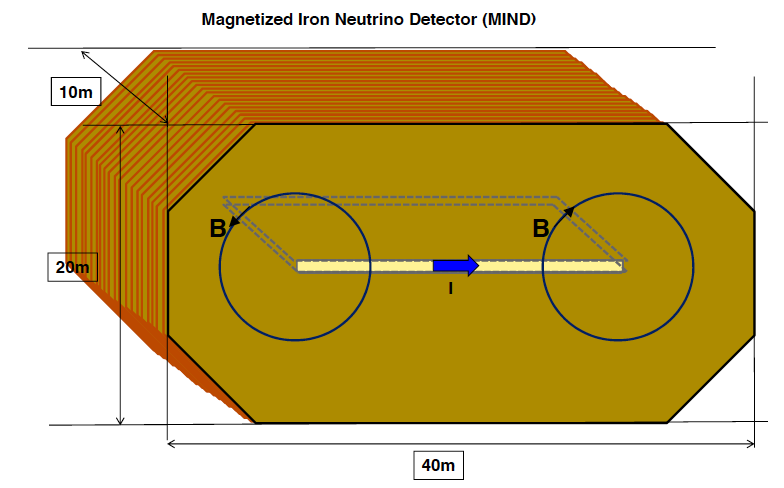
\includegraphics[width=100mm]{Chapter2/figures/mindFDdesign.png}
\caption{The sketch of the potential MIND design. Image from \cite{lbnoInternal}.}
\label{fig:mindFD}
\end{center}
\end{figure}

\begin{figure}[htbp]
\begin{center}
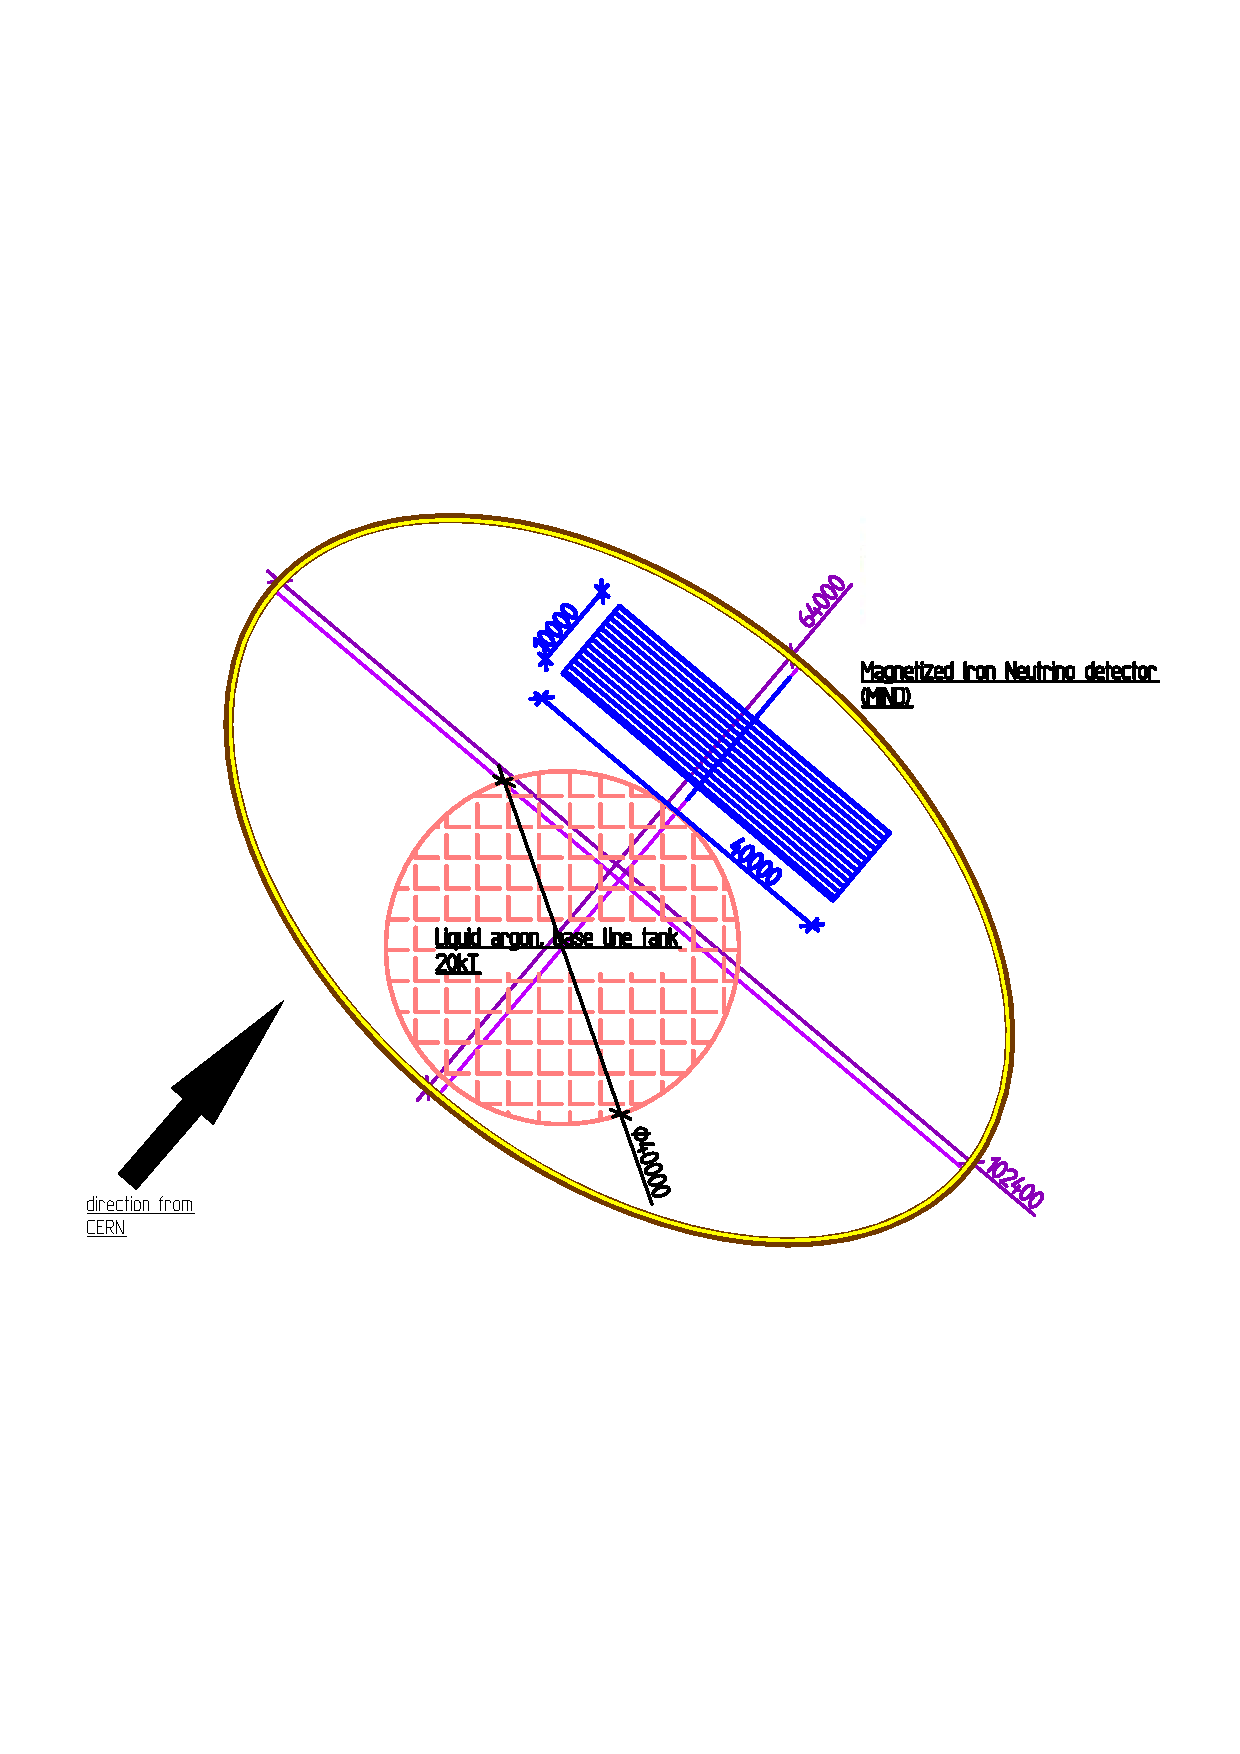
\includegraphics[width=100mm]{Chapter2/figures/glacierMindLayout.pdf}
\caption{The proposed layout for both the GLACIER and MIND far detectors with dimensions in mm. Image from \cite{lbnoInternal}.}
\label{fig:glacierMindLayout}
\end{center}
\end{figure}

\section{The Pyh\"asalmi Site}
The site itself is currently a working mine but is planned to be decommissioned around 2018 enabling the mine to be fully devoted to the experiment after this date. The mine has excellent existing infrastructure, with excavated roads allowing vehicles to drive to the maximum depth of the mine. The existing infrastructure layout is shown in figure \ref{fig:mineLayout}. Excavations will still be need to be performed in order to host the detectors however, with costs estimated at $\sim$100 million EUR \cite{lbnoInternal}. 

\begin{figure}[htbp]
\begin{center}
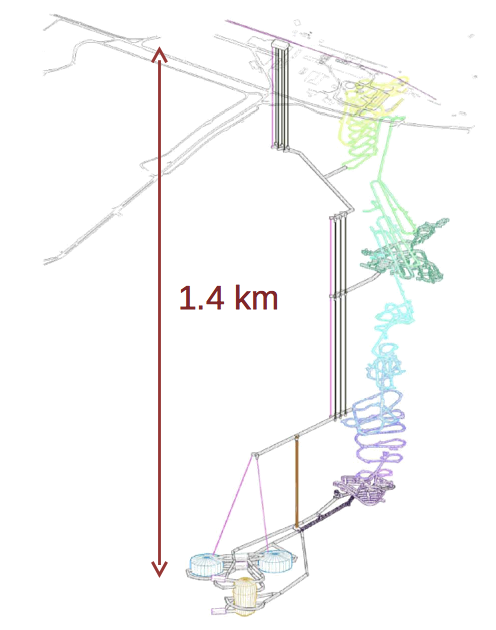
\includegraphics[width=60mm,height=80mm]{Chapter2/figures/mineLayout.png}
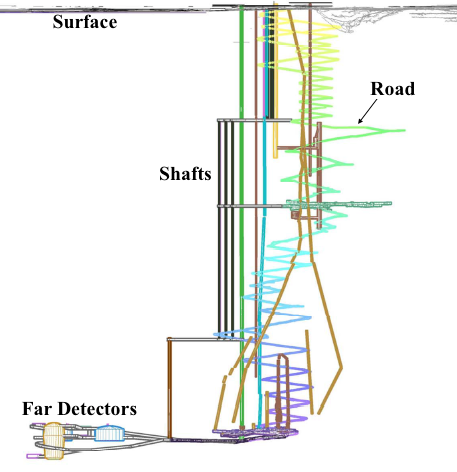
\includegraphics[width=60mm,height=80mm]{Chapter2/figures/mineLayout2.png}
\caption{The current layout of the Pyh\"asalmi mine with possible implementation of the detectors at a depth of 1400 m. Image from \cite{lbnoInternal}.}
\label{fig:mineLayout}
\end{center}
\end{figure}

%\section{Other Proposed Long Baseline Experiments}
%LAGUNA-LBNO is not the only current long baseline experiment proposed, it is however the only proposed experiment that covers such a baseline and can alone determine the mass hierarchy to > 5$\sigma$. Other potential experiments are Long Baseline Neutrino Experiment (LBNE)\cite{LBNE} in the United States and Hyper-K (in Japan)\cite{hyperK} to name the big two contenders. 
